\documentclass[conference]{IEEEtran}
\IEEEoverridecommandlockouts
% The preceding line is only needed to identify funding in the first footnote. If that is unneeded, please comment it out.
\usepackage{cite}
\usepackage{amsmath,amssymb,amsfonts}
\usepackage{algorithmic}
\usepackage{graphicx}
\usepackage{textcomp}
\usepackage{xcolor}
\usepackage{multirow}
\def\BibTeX{{\rm B\kern-.05em{\sc i\kern-.025em b}\kern-.08em
    T\kern-.1667em\lower.7ex\hbox{E}\kern-.125emX}}
\begin{document}

\title{Analisis Kualitas Signal Wi-Fi Berbasis ESP-8266
Dengan Notifikasi Bot Telegram pada Institut
Teknologi Batam}


\author{\IEEEauthorblockN{Raja Muhammad Fikri\IEEEauthorrefmark{1}, Farhan Ghulam\IEEEauthorrefmark{2}, Hani Khairiyah\IEEEauthorrefmark{4}}
\IEEEauthorblockA{\textit{Fakultas Teknologi Informasi} \\
\textit{Teknik Komputer}\\ 
\textit{Institut Teknologi Batam} \\
Batam, Indonesia\\
Email: (\IEEEauthorrefmark{1}1822013, \IEEEauthorrefmark{2}1822014, \IEEEauthorrefmark{4}1922001) @student.iteba.ac.id}
}

\maketitle

\begin{abstract}
Wi-Fi tentu saja tidak terlepas dari yang dinamakan sinyal,
kuat lemahnya sinyal mempengaruhi kemampuan komunikasi nirkabel.
Untuk mengukur kuat sinyal Wi-Fi dibutuhkan alat ukur yang \textit{optical power meter} atau juga disebut \textit{radio frequency power meter}. Penulis berinovasi
dengan mengkombinasikan prinsip kerja \textit{ptical power meter} dengan prinsip kerja \textit{Internet of Things}. Yang mana alat ini berfungsi memindai SSID, RSSI serta menggolongkan kuat sinyal dalam empat kategori, yaitu : \textit{Excellent, Good, Fair, Poor}. Alat ini bekerja dengan memanfaatkan telegram bot untuk bisa mengirimkan hasil pemindaian Wi-Fi. Dalam penerapannya penulis menggunakan mikrokontroler \textit{ESP-8266} serta bot telegram dengan server milik BotFather.
\end{abstract}

\begin{IEEEkeywords}
\textit{Wi-Fi, ESP-8266, BotFather, SSID, RSSI}
\end{IEEEkeywords}

\section{PENDAHULUAN}
Perkembangan teknologi semakin tidak terbendung, terlebih pada aspek
jaringan dan komunikasi. Berkembangnya jaringan nirkabel Wi-Fi menjadi trobosan yang membuka jalan untuk pengembangan teknologi berikutnya. Membahas mengenai jaringan nirkabel Wi-Fi tentu saja tidak terlepas dari yang dinamakan sinyal, kuat lemahnya sinyal mempengaruhi kemampuan komunikasi nirkabel. Untuk mengukur kuat sinyal Wi-Fi dibutuhkan alat ukur yang \textit{optical power meter} atau juga disebut \textit{radio frequency power meter}.

Institut Teknologi Batam memanfaatkan jaringan wifi sebagai salah satu fasilitas untuk penunjang pelaksanaan kegiatan perkuliahan mahasiswa dan akademik di lingkup Institut Teknologi Batam. Namun dengan banyaknya mahasiswa Institut Teknologi Batam yang kurang lebih sekitar 500 orang mengakibatkan akses internet ke jaringan internet menjadi lambat. Selain itu, ada beberapa fakultas di beberapa lantai tidak mendapat sinyal wifi atau mendapat sinyal yang lemah sehingga mahasiswa tidak dapat menikmati jaringan intenet dengan baik.

Oleh karna itu penulis berinovasi dengan mengkombinasikan prinsip kerja \textit{optical power meter} dengan prinsip kerja \textit{Internet of Things}. Yang mana alat ini berfungsi memindai SSID, RSSI serta menggolongkan kuat sinyal dalam empat kategori, yaitu : \textit{Excellent, Good, Fair, Poor}. Alat ini bekerja dengan memanfaatkan telegram bot untuk mengirimkan hasil pemindaian Wi-Fi. Dalam penerapannya penulis menggunakan mikrokontroler \textit{ESP-8266} serta bot \textit{telegram} dengan server milik \textit{BotFather}. Mengukur kualitas sinyal dapat diketahui dengan melihat nilai parameter performa jaringan wifi yaitu,
\begin{enumerate}
    \item Kuat Sinyal (\textit{Signal Strength}) Kualitas sinyal menentukan handal tidaknya suatu Wi-Fi, artinya semakin kuat sinyal maka semakin baik dan handal konektivitasnya. Kekuatan sinyal yang dipancarkan oleh perangkat Wi-Fi atau suatu \textit{Access Point} sangat dipengaruhi oleh infrastruktur yang membangun access point tersebut.
    
    \begin{table}[htbp]
        \caption{SKALA TINGKATAN LEVEL \textit{SIGNAL}}
        \label{tab1}
        \centering
        \begin{tabular}{|c|c|c|c|}
        \hline
        \textbf{Nilai Kuat Sinyal} & \multirow{2}{*}{\textbf{Kategori}} & \multirow{2}{*}{\textbf{Keterangan}} & \textbf{Tingkat Kuat Sinyal} \\
        \textbf{(dBm)} &  &  & \textbf{(Bar Sinyal)}\\
        \hline
        -35 s/d 60 & Excellent & Sangat Baik & 4 \\ \hline
        -60 s/d -70 & Good & Baik & 3 \\ \hline
        -71 s/d -85 & Fair & Buruk & 2 \\ \hline
        -85 s/d -95 & Poor & Sangat Buruk & 1\\
        \hline
        \end{tabular}
    \end{table}
    
    \item \textit{Signal to Noise Ratio (SNR)}\\
    \textit{Signal to Noise Ratio (SNR)} adalah rasio perbandingan antara sinyal yang diterima dengan gangguan (derau) sekitar dengan satuan desibel (dB). \textit{Signal to Noise Ratio} merupakan kunci penentu apakah jaringan \textit{wireless} memiliki performa bagus atau tidak. Semakin tinggi nilai , maka semakin bagus performa jaringan tersebut.
    
    \begin{table}[htbp]
        \caption{SKALA SNR}
        \label{tab2}
        \centering
        \begin{tabular}{|c|c|c|}
        \hline
        \textbf{Nilai SNR} & \textbf{Kategori} & \textbf{Keterangan} \\
        \hline
        \multirow{2}{*}{$>$40 dB} & \multirow{2}{*}{\textit{Excellent}} & Cepat terkoneksi, \textit{Troughput}  \\ 
        & &  maksimal dan stabil \\
        \hline
        \multirow{2}{*}{25 dB s/d 40 dB} & \textit{Very Good} &  Terkoneksi baik, \\ 
        & \textit{Signal} & \textit{Troughput} maksimal  \\ \hline
        \multirow{2}{*}{15 dB s/d 25 dB} & \multirow{2}{*}{\textit{Low Signal}} &  Terkoneksi baik, \\
        & & \textit{throughput} tidak maksimal \\
        \hline
        \multirow{2}{*}{10 dB s/d 15 dB} & \textit{Very Low} &  Koneksi tidak  terlalu \\ 
        & \textit{Signal} & stabil, \textit{throughput} rendah \\
        \hline
       \multirow{2}{*}{5 dB s/d 10 dB} & \multirow{2}{*}{\textit{No Signal}} & koneksi sangat tidak stabil, \\ 
        & & \textit{throughput} sangat rendah \\
        \hline
        \end{tabular}
    \end{table}
    
\end{enumerate}

\section{LANDASAN TEORI}

\subsection{\textit{Bot Telegram}}
Fitur Bot ini telah diluncurkan di aplikasi \textit{Telegram} pada tahun 2015 lalu.
\textit{Telegram} Bot ini merupakan sebuah singkatan dari robot, yang dengan kata lain mempunyai arti sebagai mesin yang dapat menanggapi sebuah pesan user secara otomatis untuk pekerjaan yang kita inginkan. Umumnya, bot beroperasi menggunakan internet atau yang disebut juga dengan internet bot atau komputer bot. Dengan begitu, bot dapat dimanfaatkan untuk membantu mempermudah pekerjaan manusia. Seperti memberikan layanan pelanggan otomatis, mencari konten secara online, hingga membantu pengoptimalan mesin telusur. Pada penelitian ini penulis menggunakan layanan \textit{development bot telegram} yang bernama \textit{BotFather} untuk mengembangkan alat ukut kuat sinyal Wi-Fi berbasis \textit{ESP-8266} sebagai platform notifikasi pesan hasil pemindaian. \textit{BotFather} dipilih karena memiliki keunggulan yaitu mudah dalam pembuatannya dimana kita tidak perlu membuat server sendiri karena \textit{BotFather} telah menyediakan server bagi penggunanya, serta kemudahan akses \textit{ESP-8266} sehingga memperingkas algoritma dan mengurangi kegagalan data komunikasi.

\subsection{\textit{ESP-8266}}
\textit{ESP-8266} merupakan sebuah mikrokontroller yang sering digunakan untuk
perangkat \textit{Internet of Things} atau yang biasa disebut IoT. Mikrokontroller buatan Espressif Systems ini mempunyai fitur yang cukup lengkap dan mudah
digunakan. Salah satu fitur yang paling menonjol adalah modul Wi-Fi. Daya
transmisi +20 dBm dalam mode 802.11b. Mendukung mode \textit{Client, Station} (STA), \textit{Access Point} (AP), dan STA+AP. Pada penelitian ini penulis menggunakan mode \textit{Client} dan \textit{Station}. Yang mana mode Client mampu mengubungkan \textit{ESP-8266} ke internet untuk bisa terhubung dan menerima pesan
dari bot \textit{telegram}. Sedangkan mode \textit{Station} mampu menjadikan \textit{ESP-8266} sebagai mesin pemindai Wi-Fi dimana hasil pemindaian berupa SSID dan RSSI(dBm).

\section{METODE PENELITIAN}
\subsection{Waktu dan Tempat}
Penelitian ini dilaksanakan di lingkungan indoor dan outdoor Institut
Teknologi Batam. Waktu penelitian, pengujian, dan analisis secara umum
dilakukan 1 Juli 2022 sampai 1 Agustus 2022.

\subsection{Alat dan Bahan Penelitian}
Alat dan Bahan yang digunakan pada penelitian ini sebagai berikut:
\begin{table}[htbp]
        \caption{DAFTAR ALAT}
        \label{tab3}
        \centering
        \begin{tabular}{|c|c|c|c|}
        \hline
        \textbf{No} & \textbf{Nama Alat} & \textbf{Spesifikasi}& \textbf{Keterangan} \\
        \hline
        \multirow{2}{*}{1.} & \multirow{2}{*}{Laptop} & \multirow{2}{*}{ASUS X450JN Intel-i7} & Digunakan untuk \\ 
        & & & membuat program \\
        \hline
        \end{tabular}
\end{table}

\begin{table}[htbp]
        \caption{DAFTAR BAHAN}
        \label{tab4}
        \centering
        \begin{tabular}{|c|c|c|c|}
        \hline
        \textbf{No} & \textbf{Nama Bahan} & \textbf{Spesifikasi}& \textbf{Keterangan} \\
        \hline
        \multirow{2}{*}{1.} & \multirow{2}{*}{Aplikasi \textit{Arduino} IDE} & \multirow{2}{*}{Versi 1.8.18} & Digunakan untuk \\ 
        & & & pemrograman \\
        \hline
         \multirow{2}{*}{2.} & \multirow{2}{*}{Aplikasi \textit{Telegram}} & \multirow{2}{*}{Versi 4.0.2} & Digunakan untuk \\ 
        & & & \textit{monitoring} wifi \\
        \hline
        \end{tabular}
\end{table}  
   
\begin{table}[htbp]
        \caption{DAFTAR KOMPONEN}
        \label{tab5}
        \centering
        \begin{tabular}{|c|c|c|c|}
        \hline
        \textbf{No} & \textbf{Nama Komponen} & \textbf{Spesifikasi}& \textbf{Keterangan} \\
        \hline
        \multirow{3}{*}{1.} & \multirow{3}{*}{\textit{NodeMcu Esp-8266}} & \multirow{3}{*}{12-e} & Digunakan untuk \\
        & & & pemindaian dan \\
        & & & \textit{scanning} wifi \\
        \hline
         \multirow{3}{*}{2.} & \multirow{3}{*}{Kabel Micro USB} & \multirow{3}{*}{Type B} & Digunakan untuk \\ 
        & & & menghubungkan \\
        & & & \textit{Hardware dan Software} \\
        \hline
        \end{tabular}
\end{table}

%\vspace{2\baselineskip}
\subsection{Metode Penelitian}
Langkah-langkah penelitian ini dapat dilihat pada diagram alir penelitian
dibawah ini.\\

\begin{figure}[htbp]
\centerline{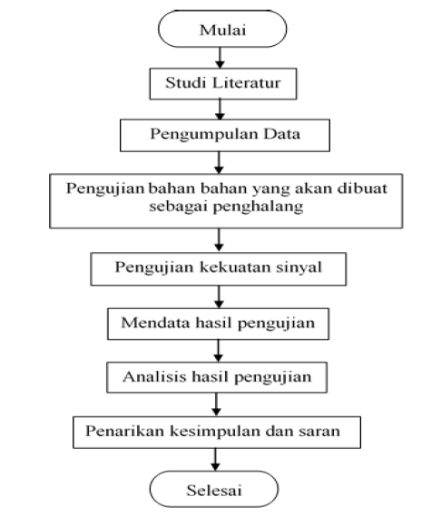
\includegraphics[width=8cm, height=10.3cm]{gambar.png}}
\caption{Diagram Alir Penelitian}
\label{fig}
\end{figure}


\section{ANALISA DAN PENGUJIAN}
\subsection{Tahap Analisa}
Ada beberapa macam hal yang dapat mengganggu perederan sinyal wifi
untuk dapat terdeteksi pada perangkat \textit{NodeMcu Esp-8266} yang menyebabkan
terhambatnya aktifitas \textit{searching or browsing} di internet, hal tersebut
diantaranya :
\begin{enumerate}
    \item Penyerapan/Peredaman Sinyal (\textit{Bsorption})\\
    Seperti diketahui semakin besar Amplitudo gelombang (\textit{Power}) Semakin jauh sinyal wifi dapat memancar. Ini baik karena dapat menghemat \textit{access point} dan menjangkau lebih luas. Dengan mengurangi besar amplitudo (\textit{Power}) suatu sinyal, maka jarak jangkauan sinyal wifi tersebut akan berkurang. Faktor yang mempengaruhi transmisi \textit{wireless} dengan mengurangi amplitudo (\textit{Power}). Efek dari Penyerapan adalah panas. Contohnya: tembok, kaca, karpet.
    \item Pemecahan Sinyal (\textit{Scattering})\\
    Isu dari pemecahan sinyal terjadi saat sinyal di kirim dalam banyak arah. Hal ini dapat disebabkan oleh beberapa objek yang dapat memantulkan sinyal dan ujung yang lancip, seperti partikel debu di air dan udara. Ilustrasinya adalah menyinari lampu ke pecahan kaca. Cahaya akan dipantulkan ke banyak arah dan menyebar.
    \item Pembelokan Sinyal (\textit{Refraction})\\
    Refraction adalah perubahan arah, atau pembelokan dari sinyal wifi disaat sinyal melewati sesuatu yang beda massa nya. Sebagai contoh sinyal yang melewati segelas air, sinyal ada yang di pantulkan dan ada yang dibelokkan.
\end{enumerate}

\subsection{Tahap Pengujian}
Pada tahap pengujian ini dilakukan dengan cara yang sederhana terhadap kekuatan sinyal. Setiap tahapan pengujian dilakukan secara bergantian agar mendapatkan hasil yang maksimal. Berikut ini adalah 3 tahapan dimulai nya pengujian:
\begin{enumerate}
    \item Pengujian pengaruh material package terhadap kemampuan penerimaan sinyal wifi. Pengujian ini berguna untuk mendapatkan hasil dan analisa pengaruh material \textit{package} terhadap kemampuan penerimaan sinyal wifi, mendapatkan nilai penerimaan sinyal tertinggi dan terendah dari suatu material, dan mendapatkan material mana yang paling cocok untuk digunakan.
    \item Pengujian pengaruh gangguan elektromagnetik perangkat elektronik terhadap kemampuan penerimaan sinyal wifi. Pengujian ini berguna untuk mendapatkan hasil dan analisa pengaruh perangkat elektronik terhadap kemampuan penerimaan sinyal wifi, mendapatkan nilai penerimaan sinyal tertinggi dan terendah dari suatu pengaruh alat elektronik di sekeliling lokasi pengujian, dan perangkat elektronik mana yang paling mengganggu terhadap penerimaan sinyal.
    \item Pengujian pengaruh jam operasional terhadap kemampuan penerimaan sinyal wifi. Pengujian ini berguna agar mengetahui korelasi antara penerimaan sinyal dan tingkat ramainya aktifitas di jam tertentu, mendapatkan nilai penerimaan sinyal tertinggi dan terendah pada jam tertentu.
\end{enumerate}

\section{HASIL DAN PEMBAHASAN}
Pada bagian ini akan dibahas mengenai hasil yang didapatkan dari tahap analisa dan beberapa tahap pengujian kekuatan sinyal yang sudah dilakukan.
\subsection{Hasil Pengukuran}

\begin{table}[htbp]
        \caption{HASIL PENGUJIAN PENGARUH MATERIAL \textit{PACKAGE}}
        \label{tab6}
        \centering
        \begin{tabular}{|c|c|c|c|c|}
        \hline
        \multirow{3}{*}{\textbf{No}} & \multirow{3}{*}{\textbf{SSID}} & \multicolumn{3}{|c|}{\textbf{RSSI(dBm)}} \\
        \cline{3-5} 
         & & \textbf{\textit{Package}}& \textbf{\textit{Package}} & \textbf{\textit{Package}}\\
         & & \textbf{Plastik} & \textbf{Aluminium} & \textbf{Kaca}\\
        \hline
        1 & DOSEN ITEBA 2 & -54 & -80 & -48 \\ \hline
        2 & STUDENT ITEBA & -54 & -80 & -49 \\ \hline
        3 & STUDENT BTP & -55 & -79 & -50 \\ \hline
        4 & DOSEN BTP 2 & -54 & -80 & -48 \\
        \hline
        \end{tabular}
\end{table}

Pada Table \ref{tab6} diatas, dapat dilihat bahwa SSID yang ada di Institut Teknologi Batam berdasarkan hasil kuat sinyal wifi yang diterima oleh \textit{NodeMcu Esp-8266} dengan notifikasi \textit{Telegram} terhadap pengujian pengaruh material \textit{package} plastik diperoleh hasil rata-rata sebesar -55 (dBm) dengan kualitas sinyal dalam kategori sangat baik, sedangkan pengujian pengaruh material \textit{package} aluminium diperoleh hasil rata-rata sebesar -80 (dBm) dengan kualitas sinyal dalam kategori buruk, sedangkan untuk pengujian pengaruh material \textit{package} kaca diperoleh hasil rata-rata sebesar -50 (dBm) dengan kualitas sinyal dalam kategori sangat baik.

\begin{table}[htbp]
        \caption{HASIL PENGUJIAN PENGARUH PERANGKAT ELEKTRONIK}
        \label{tab7}
        \centering
        \begin{tabular}{|c|c|c|c|c|}
        \hline
        \multirow{3}{*}{\textbf{No}} & \multirow{3}{*}{\textbf{SSID}} & \multicolumn{3}{|c|}{\textbf{RSSI(dBm)}} \\
        \cline{3-5} 
         & & \textbf{Jaringan}& \multirow{2}{*}{\textbf{Laptop}} & \textbf{Lab}\\
         & & \textbf{seluler} &  & \textbf{Elektronika}\\
        \hline
        1 & DOSEN ITEBA 2 & -55 & -54 & -52 \\ \hline
        2 & STUDENT ITEBA & -55 & -56 & -52 \\ \hline
        3 & STUDENT BTP & -53 & -54 & -53 \\ \hline
        4 & DOSEN BTP 2 & -54 & -55 & -53 \\
        \hline
        \end{tabular}
\end{table}

Pada Table \ref{tab7} diatas, dapat dilihat bahwa SSID yang ada di Institut Teknologi Batam berdasarkan hasil kuat sinyal wifi yang diterima oleh \textit{NodeMcu Esp-8266} dengan notifikasi \textit{Telegram} terhadap pengujian pengaruh perangkat elektronik seperti jaringan seluler diperoleh hasil rata-rata sebesar -55 (dBm) dengan kualitas sinyal dalam kategori sangat baik, sedangkan pengujian pengaruh perangkat elektronik seperti laptop diperoleh hasil rata-rata sebesar -56 (dBm) dengan kualitas sinyal dalam kategori sangat baik, dan sedangkan pengujian pengaruh perangkat elektronik di lab elektronika diperoleh hasil rata-rata sebesar -53 (dBm) dengan kualitas sinyal dalam kategori sangat baik.

\begin{table}[htbp]
        \caption{HASIL PENGUJIAN PENGARUH JAM OPERASIONAL}
        \label{tab8}
        \centering
        \begin{tabular}{|c|c|c|c|c|}
        \hline
        \multirow{2}{*}{\textbf{No}} & \multirow{2}{*}{\textbf{SSID}} & \multicolumn{3}{|c|}{\textbf{RSSI(dBm)}} \\
        \cline{3-5} 
         & & \textbf{08.00}& \textbf{12.00} & \textbf{19.00}\\
        \hline
        1 & DOSEN ITEBA 2 & -53 & -79 & -55 \\ \hline
        2 & STUDENT ITEBA & -55 & -77 & -57 \\ \hline
        3 & STUDENT BTP & -54 & -76 & -55 \\ \hline
         4 & DOSEN BTP 2 & -55 & -81 & -55 \\
       \hline
        \end{tabular}
\end{table}



Pada Table \ref{tab8} diatas, dapat dilihat bahwa SSID yang ada di Institut Teknologi Batam berdasarkan hasil kuat sinyal wifi yang diterima oleh \textit{NodeMcu Esp-8266} dengan notifikasi \textit{Telegram} terhadap pengujian pengaruh jam operasional pada jam 08.00 pagi diperoleh hasil rata-rata sebesar -55 (dBm) dengan kualitas sinyal dalam kategori sangat baik, sedangkan pengujian pengaruh jam operasional pada jam 12.00 siang diperoleh hasil rata-rata sebesar -80 (dBm) dengan kualitas sinyal dalam kategori buruk, sedangkan untuk pengujian pengaruh jam operasional pada jam 19.00 malam diperoleh hasil rata-rata sebesar -56 (dBm) dengan kualitas sinyal dalam kategori sangat baik.


\section{KESIMPULAN}
Berdasarkan hasil analisa simulasi \textit{Scanning} kekuatan sinyal wifi di Institut Teknologi Batam, penulis membuat beberapa kesimpulan yaitu :
\begin{enumerate}
    \item Proses \textit{Wifi Signal Analysis} yang sudah dilakukan di Institut Teknologi Batam menggunakan \textit{NodeMcu Esp-8266} dengan notifikasi bot \textit{Telegram} dapat digunakan untuk melakukan sebuah perintah yang dapat mengetahui kekuatan sinyal jaringan (dBm) di setiap SSID wifi yang berada di Institut Teknologi Batam dan sekitarnya.
    \item Terjadinya pengurangan penguatan sinyal wifi jika berdasarkan pengujian pengaruh material \textit{package} aluminium, dan kategori kuat sinyal yang didapat adalah buruk.
    \item Pada proses pengujian pengaruh perangkat elektronik didapatkan hasil kuat sinyal kategori sangat baik dan tidak memberikan efek terhadap pelemahan sinyal wifi.
    \item Pada proses pengujian pengaruh jam operasional terhadap kuat sinyal wifi terdapat pelemahan sinyal wifi pada jam 12.00 siang dikarenakan aktifitas manusia sedang beristirahat makan siang di kantin Institut Teknologi Batam.
    \item Pada skala tingkatan kualitas sinyal, dapat diketahui juga kategori-kategori kuat sinyal jaringan seperti: \textit{Excellent, Good, Fair}, dan \textit{Poor}.
    \item Adapun faktor - faktor penyebab koneksi tidak stabil, sering putus koneksi dan terkadang no sinyal yaitu pengguna yang melebihi batas jarak kemampuan \textit{Access Point}.
\end{enumerate}


\end{document}
